\documentclass[12pt]{article}

\usepackage{lmodern}
\usepackage[T1]{fontenc}
\usepackage[spanish,activeacute]{babel}
\usepackage[utf8]{inputenc}
\usepackage{mathtools}
\usepackage{enumerate}
\usepackage{amsthm}
\usepackage{amssymb}
\usepackage[hidelinks]{hyperref}
\usepackage{anysize}
\usepackage{listings}
\usepackage{float}
\usepackage{hyperref}
\usepackage{graphicx}

\marginsize{2cm}{2cm}{2cm}{2cm}

\lstset{ %
escapeinside=||,
language=python,
basicstyle=\small}

\title{Metaheur\'isticas:\\
 Pr\'actica 2.b: B\'usquedas Multiarranque para el Problema de Selección de Características}
\author{Anabel G\'omez R\'ios.\\
 DNI: 75929914Z.\\
 E-mail: anabelgrios@correo.ugr.es}


\begin{document}
\maketitle

\begin{center}
Curso 2015-2016\\

Problema de Selección de Características.\\ 

Grupo de prácticas: Viernes 17:30-19:30\\

Quinto curso del Doble Grado en Ingeniería Informática y Matemáticas.\\
\textit{ }\\
\end{center}

Algoritmos considerados:
\begin{enumerate}
\item Búsqueda Multiarranque Básica
\item GRASP
\item Búsqueda Local Reiterada
\end{enumerate}

\newpage

\tableofcontents

\newpage

\section{Descripción del problema}
Queremos obtener un sistema que permita clasificar un conjunto de objetos en unas determinadas clases que conocemos previamente. Para ello disponemos de una muestra de dichos objetos ya clasificados y una serie de características para cada objeto.\\

El problema es, por tanto, construir un clasificador que se comporte lo suficientemente bien fuera de la muestra de la que disponemos, es decir, que clasifique bien nuevos datos. Para hacer esto, lo que hacemos es particionar la muestra en dos subconjuntos, uno que utilizaremos de entrenamiento para que el clasificador aprenda y otro que utilizaremos para test, es decir, para ver cómo de bien se comporta el clasificador que hemos obtenido con el primer subconjunto fuera de los datos de entrenamiento. Además haremos distintas particiones, en concreto 5, y construiremos un clasificador para cada una de ellas. Las particiones serán además proporcionadas (habrá el mismo número de muestras de una clase en el conjunto de entrenamiento y en el de test). Podemos comprobar cómo de bien se comporta cada clasificador porque sabemos en realidad las clases de los objetos que tenemos en la muestra y podemos comparar las verdaderas clases con las que el clasificador obtiene suponiendo que no dispusiéramos de ellas.\\
Buscamos pues en todo momento optimizar la tasa de acierto del clasificador.\\
Vamos a utilizar además validación cruzada: es decir, para cada partición en dos subconjuntos primero uno será el de entrenamiento y el otro el de test y después les daremos la vuelta y volveremos a construir un clasificador. La calidad por tanto de cada algoritmo será la media de los porcentajes de clasificación (la tasa de acierto) para estas 10 particiones.\\

Nos queda describir cómo aprende el clasificador con los datos de entrenamiento. Ya que podemos llegar a tener muchas características de las cuales algunas podrían ser poco o nada significantes, lo que hacemos es elegir un subconjunto de características que describan bien los datos de entrenamiento, de forma que en los datos de test sólo tenemos en cuenta este subconjunto de características a la hora de deducir cuál es la clase de cada nuevo dato. Para esta "deducción" vamos a utilizar la técnica de los 3 vecinos más cercanos (3-NN): buscamos para cada dato los tres vecinos más cercanos en el conjunto de entrenamiento (si el mismo dato al que le vamos a calcular la clase pertenece al conjunto de entrenamiento tenemos que sacarlo previamente del conjunto de entrenamiento. Esto es lo que se llama \textit{leave one out}) teniendo en cuenta las características seleccionadas hasta el momento, consultamos las clases de estos tres vecinos, nos quedamos con la clase que más veces aparezca (o, en caso de empate, con la clase del vecino más cercano) y ésta será la clase del dato. Para obtener la tasa de acierto lo que hacemos es repetir esto para todos los datos, comparar estas clases con las reales y contar el número de veces que acierta.\\

El cómo exploramos el espacio de búsqueda hasta encontrar la mejor solución (el subconjunto de características que da mayor tasa de acierto) es en lo que se diferencian los distintos algoritmos que vamos a ver en esta práctica.

\newpage

\section{Descripción de la aplicación de los algoritmos empleados al problema}
El primer paso común a todos los algoritmos es normalizar los datos de los que disponemos por columnas (es decir, por características) de forma que todas se queden entre 0 y 1 y no haya así preferencias de unas sobre otras.\\

A continuación se genera una solución inicial, que en el caso de los algoritmos SFS y GRASP serán todas las características a \textit{False} y se irán añadiendo en base a distintos criterios y en el caso de los algoritmos BMB e ILS serán aleatorias. Después, se irán generando vecinos de esta solución (veremos que algunos mutan, otros optimizan con búsqueda local, etc.) y nos quedaremos con la mejor solución obtenida en todos los casos.\\

Todos los algoritmos tienen una condición de parada común (excepto SFS), que es repetir la generación de solución inicial y posterior optimización (el bucle interno) 25 veces.

\subsection{Esquema de representación de soluciones}
La representación elegida para las soluciones ha sido la binaria: un vector de $N$ posiciones, donde $N$ es el número de características, en el que aparece \textit{True} o \textit{False} en la posición $i$ según si la característica $i$-ésima ha sido seleccionada o no, respectivamente. Esta representación es la más sencilla y cómoda cuando no hay restricciones sobre el número de características a elegir, es decir, el número de características que se han de elegir lo aprende cada algoritmo, como es el caso de los algoritmos que vamos a utilizar.

\subsection{3-NN}
Como hemos comentado, la técnica para clasificar que vamos a utilizar en todos los algoritmos será el 3NN. Consiste en considerar, para cada dato, la distancia euclídea entre el dato y todos los demás, es decir, entre las características de los datos (excluyéndose él mismo en caso de que estuviéramos preguntando por algún dato dentro del conjunto de entrenamiento) y quedarnos con las clases de los 3 con la distancia más pequeña. La clase del dato en cuestión será de estas tres la que más se repita o, en caso de empate, la clase que corresponda al vecino más cercano.\\
En cada momento la distancia euclídea se calcula teniendo en cuenta las características que están seleccionadas en el momento, por lo que no podemos tener una matriz fija de distancias, hay que ir calculándolas sobre la marcha.

\subsection{Función de evaluación}
La función de evaluación será el rendimiento promedio de un clasificador 3-NN en el conjunto de entrenamiento: calcularemos la tasa para cada dato dentro del conjunto de entrenamiento haciendo el leave one out descrito anteriormente y nos quedaremos con la media de las tasas obtenidas. El objetivo será por tanto maximizar esta función.
La tasa se calcula como 100*(nº instancias bien clasificadas / nº total de instancias).\\

El pseudo-código es el siguiente:\\
\begin{lstlisting}
Obtener el subconjunto de entrenamiento que se va a tener en cuenta seg|ú|n 
las caracter|í|sticas que se est|é|n considerando.
Para cada dato:
   Se saca del conjunto de entrenamiento (leave one out)
   Se calcula la tasa para este dato con el clasificador 3NN
   Se acumula la tasa al resto de tasas
Se divide la acumulaci|ó|n de tasas entre el cardinal del conjunto y se devuelve
\end{lstlisting}
La función que hace esto la llamaremos \texttt{CalcularTasa(conjunto, caracteristicas, knn)} donde \texttt{caracteristicas} es la máscara que nos indica cuáles estamos considerando (aquellas que estén a True), \texttt{conjunto} es el conjunto de entrenamiento y \texttt{knn} es el clasificador 3NN ya previamente entrenado con el conjunto \texttt{conjunto}.\\

En mi caso para el clasificador 3-NN he utilizado el que ha implementado mi compañero Alejandro García Montoro (de mi mismo grupo de prácticas) con python y CUDA, puesto que es mucho más eficiente.

\subsection{Operadores comunes: Generación de vecinos}
Se considerarán como vecinas todas aquellas soluciones que difieran en la pertenencia o no de una única característica (si se diferencian en más de una entonces no es vecina de la considerada). Por ejemplo, las soluciones (True, True, False) y (True, False, False) son vecinas porque se diferencian en una sola característica, la segunda.\\
\texttt{Flip} será el operador de vecino: recibe un vector que será la máscara y una posición y cambia esa posición en la máscara. El que he hecho yo además lo hace por referencia para evitar las copias e intentar mejorar en eficiencia.\\

\begin{lstlisting}
Flip(mascara, pos) |\textbf{Empezar}|:
   # Cambiar la posici|ó|n pos de la m|á|scara por su negado 
   mascara[pos] = not mascara[pos]
   |\textbf{Devolver}| mascara
Fin
\end{lstlisting}

\subsection{Proceso de generación de soluciones aleatorias}
En mi caso para la generación aleatoria de soluciones en los algoritmos BMB e ILS he utilizado la función \texttt{choice()} del módulo \texttt{random} de \texttt{numpy} para python, a la que se le puede pasar el vector de donde obtener las muestras (en mi caso un array de \textit{True} y \textit{False}) y el número de muestras a obtener (suponemos \textit{n} ahora mismo, será en cada caso el número de características). El muestreo se hace con reemplazamiento:
\begin{lstlisting}
generarSolAleatoria(n) |\textbf{Empezar}|:
	sol_aleatoria = random.choice(array([True, False]), n)
	|\textbf{Devolver}| sol_aleatoria
Fin
\end{lstlisting}

\subsection{Búsqueda Local}
El algoritmo de búsqueda local implementado ha sido el del primer mejor, es decir, exploramos los vecinos de la solución que tenemos en cada momento y en cuanto obtenemos una mejor nos quedamos con ella y empezamos a generar sus vecinos. Los vecinos se empiezan a generar por una característica aleatoria y a partir de esa característica se van cambiando las demás de forma cíclica en orden: desde la que hemos empezado hasta el final y de nuevo por el principio hasta llegar a la anterior de la primera que habíamos cambiado. Si no nos quedamos con la solución tenemos que dejar la característica que habíamos cambiado como estaba y si nos la quedamos porque tiene una mejor tasa dejamos de generar vecinos de la solución que teníamos, la cambiamos por este mejor vecino y pasamos a generar vecinos de la nueva solución. El algoritmo para cuando da una pasada entera a los vecinos y no ha encontrado una mejor solución que la que tenía.\\

Veamos el pseudocódigo.\\
\texttt{generarSecuencia(tamaño)} será la función que devuelve el orden en el que se recorrerá el vecindario: empieza desde un número aleatorio (menor que el número de características) y de ahí en orden hasta el total de características y empieza de nuevo hasta el número que se ha generado al principio. Esta función se llamará cada vez que actualicemos la solución y haya que explorar un vecindario nuevo.\\
Al algoritmo le pasamos como parámetros los datos de entrenamiento, las clases de los datos y el objeto knn que habremos creado previamente entrenándolo con esos datos y clases.
\begin{lstlisting}
busquedaLocal(datos, clases, knn) |\textbf{Empezar}|:
   caract = soluci|ó|n aleatoria inicial
   tasa actual = calcularTasa(datos, caract, knn)
   
   while haya mejora en el vecindario y haya menos de 15000 evaluaciones
    hacer:
      
      posiciones = generarSecuencia(tam(caract))
      for j en posiciones y mientras vuelta_completa = False y haya menos
       de 15000 evaluaciones hacer:
         Flip(caract, j)  # Generamos vecino
         calcularTasa(datos, caract, knn)
         if la tasa del vecino es mejor que la actual:
            actualizamos la tasa actual
            vuelta_completa = False # hemos encontrado mejora antes de
             # generar todos los vecinos, salimos del bucle y empezamos a 
             # generar vecinos de la nueva soluci|ó|n
         
         else, volvemos a la antigua soluci|ó|n:
            Flip(caract, j)
            
         if not vuelta_completa:
            vuelta_completa = True
      Fin for
   
   Fin while
   
   |\textbf{Devolver}| caract y tasa actual
Fin
   
\end{lstlisting}

\newpage

\section{Descripción de los algoritmos}

\subsection{Búsqueda Multiarranque Básica (BMB)}

Este algoritmo consiste en generar 25 soluciones aleatorias y optimizarlas con el algoritmo de Búsqueda Local que acabamos de comentar.\\
El pseudocógido es el siguiente:
\begin{lstlisting}
busquedaMultiBasica(clases, conjunto, knn) |\textbf{Empezar}|:
   for i entre 0 y 24:
      sol_aleatoria = generarSolAleatoria(num_caracteristicas)
      sol_actual, tasa_actual = busquedaLocal(clases, conjunto, knn)
		
      if tasa_actual > mejor_tasa:
         # Actualizar la mejor tasa y la mejor soluci|ó|n
         mejor_sol = sol_actual
         mejor_tasa = tasa_actual
      Fin
   Fin
   |\textbf{Devolver}| mejor_sol y mejor_tasa
Fin
\end{lstlisting}

\subsection{GRASP}

Este algoritmo es una modificación del greedy básico con el que vamos a hacer las comparaciones. Ahora, en cada paso, en lugar de elegir la mejor característica, se eligen aquellas que estén por encima de un umbral de calidad y dentro de éstas, se elige una aleatoriamente, hasta que no se obtenga mejora. Una vez tenemos construida la solución inicial greedy aleatorizada, la optimizamos con el algoritmo de Búsqueda Local. Este procedimiento lo vamos a hacer 25 veces y nos vamos a quedar con la mejor solución optimizada con Búsqueda Local de estas 25.\\

Vamos primero a poner el pseudocódigo de la función que nos va a elegir la característica siguiente en la solución greedy aleatorizada inicial en base a un umbral $\alpha$:
\begin{lstlisting}
siguienteCaracterista(clases, mascara, conjunto, alpha, knn) |\textbf{Empezar}|:
   pos = posiciones que no est|é|n ya seleccionadas en la m|á|scara
   tasas = vector vac|í|o donde guardamos las tasas de los vecinos de "mascara"
   for i en pos:
      mascara[pos[i]] = True	#Generamos el vecino
      nueva_tasa = CalcularTasa(conjunto, mascara, knn)
      tasas[i] = nueva tasa #Guardamos la tasa del vecino
      mascara[pos[i]] = False #Volvemos a la m|\textit{á}|scara original.
   Fin
   
   Calculamos el umbral como maximo-alpha*(maximo-minimo)
    donde maximo y minimo son el m|á|ximo y el m|í|nimo del vector de tasas
   
   Seleccionamos los vecinos cuya tasa est|é| por encima de ese umbral
   
   Elegimos un vecino aleatorio de los seleccionados
   
   |\textbf{Devolver}| la tasa del vecino y la posici|ó|n de la m|á|scara original
    que hay que modificar para llegar a |é|l.
Fin
\end{lstlisting}

Vamos ahora con el pseudocódigo del algoritmo GRASP, en el que vamos a hacer uso de la función anterior:
\begin{lstlisting}
GRASP(clases, conjunto, knn) |\textbf{Empezar}|:
   for i entre 0 y 24:
      caract = soluci|ó|n inicial inicializada a False
      while haya mejora:
         nueva_tasa, mejor_pos = siguienteCaracteristica(clases,
          caracteristicas, conjunto, 0.3, knn)
      
         if nueva_tasa > tasa_actual:
            Actualizamos tasa actual
            caract[mejor_pos] = True 	#Actualizamos la soluci|\textit{ó}|n
         else:
            mejora = False y paramos de a|ñ|adir caracter|í|sticas
         Fin
      Fin
   
      # Optimizamos con B|\textit{ú}|squeda Local
      sol_opt, tasa_opt = busquedaLocal(clases, conjunto, knn)
      if tasa_opt > mejor_tasa:
         Actualizar mejor_tasa y mejor_solucion
      Fin
   Fin
   
   |\textbf{Devolver}| mejor_solucion, mejor_tasa
Fin

\end{lstlisting}

\subsection{Búsqueda Local Reiterada (ILS)}

Este algoritmo consiste en generar una solución aleatoria, optimizarla con el algoritmo de Búsqueda Local, y repetir lo siguiente 24 veces: mutar la mejor solución encontrada hasta el momento y optimizarla de nuevo con Búsqueda Local. Se devolverá la mejor solución encontrada en todo este proceso.\\

Veamos primero el pseudocódigo para la función con la que vamos a mutar una solución, consistente en elegir $t$ características aleatorias de la solución y cambiarlas con el operador \texttt{Flip()}. En mi caso lo que he hecho ha sido hacer una permutación del 0 al $n$, donde $n$ es el número de características en cada caso, y cambiar las $t$ primeras posiciones del vector que he permutado en la solución.

\begin{lstlisting}
mutar(solucion, n, t) |\textbf{Empezar}|:
   mutada = copia de solucion
   pos = permutaci|ó|n del vector [0,...,n]
   for i entre 0 y t:
      Flip(mutada, pos[i])	#Cambiamos las caracter|\textit{í}|sticas aleatorias
   Fin
   |\textbf{Devolver}| mutada
Fin

\end{lstlisting}

Veamos ahora el pseudocódigo para el algoritmo ILS. Para que se mute siempre al menos una característica cuando el número de características es bajo, utilizo la función \texttt{ceil(x)} para obtener el entero por encima del valor x.
\begin{lstlisting}
ILS(clases, conjunto, knn) |\textbf{Empezar}|:
   n = n|ú|mero de caracter|í|sticas
   t = ceil(0.1*n)
   sol_aleatoria = generarSolAleatoria(n)
   # Inicializamos la mejor soluci|ón| a la optimizaci|ó|n de la aleatoria 
   mejor_sol, mejor_tasa = busquedaLocal(clases, conjunto, sol_aleatoria, knn)
   for i entre 0 y 23:
      mutada = mutar(mejor_sol, n, t)
      # Optimizamos la mutada
      sol_actual, tasa_actual = busquedaLocal(clases, conjunto, mutada, knn)
      if tasa_actual > mejor_tasa:
         Actualizamos mejor_tasa y mejor_sol
      Fin
   Fin
   |\textbf{Devolver}| mejor_sol, mejor_tasa
Fin

\end{lstlisting}

\newpage

\section{Breve descripción del algoritmo de comparación}
El algoritmo de comparación seleccionado ha sido el greedy Sequential Forward Selection (SFS), que parte de una solución inicial en la que no hay ninguna característica seleccionada y se va quedando en cada iteración con la característica con la que se obtiene la mejor tasa. El algoritmo no para mientras se encuentre mejora añadiendo alguna característica.\\
He implementado una función que me devuelve, para una máscara determinada, la característica más prometedora que se puede obtener, cuyo pseudocódigo es el siguiente:
\begin{lstlisting}
caractMasPrometedora(mascara) |\textbf{Empezar}|:
   posiciones = posiciones que no est|é|n seleccionadas de la mascara
   for i en posiciones:
      mascara[i] = True
      Se calcula la tasa con la nueva caracter|í|stica a|ñ|adida
      if nueva tasa > mejor tasa:
         Se actualiza la mejor tasa
         Se actualiza la mejor posici|ó|n
      Fin for
   |\textbf{Devuelve}| mejor tasa y mejor pos
Fin
\end{lstlisting}

Con esto, el pseudocódigo del algoritmo SFS es:
\begin{lstlisting}
algoritmoSFS(datos, clases) |\textbf{Empezar}|:
   caract = soluci|ó|n inicial inicializada a False
   tasa actual = 0
   mejora = True
   while haya mejora:
      Se calcula la tasa y la mejor posici|ó|n con caractMasPrometedora
      if nueva tasa > tasa actual:
         Se actualiza la tasa actual
         Se pone a True la caracter|í|stica en mejor posici|ó|n
      else:
         mejora = False		#No ha habido mejora: paramos
      
   Fin while
   |\textbf{Devuelve}| caract y tasa
Fin

\end{lstlisting}

\newpage

\section{Procedimiento considerado para desarrollar la práctica}
La práctica la he desarrollado en python junto con dos módulos de python: numpy y scipy (todos disponibles en Linux pero hay que instalarlos previamente), y un módulo con el 3NN con leave one out desarrollado por mi compañero Alejandro García Montoro. Numpy permite manejar arrays de forma más rápida y scipy leer ficheros en formato arff. El resto de la práctica lo he hecho yo. Para generar números aleatorios utilizo el \texttt{random} de numpy (al que le paso previamente la semilla) y para medir tiempos \texttt{time} de python.\\

Para hacer las particiones igualadas lo que he hecho ha sido quedarme, para cada clase, con los índices de los datos pertenecientes a esa clase, hacerles una permutación aleatoria, partir por la mitad y quedarme con la primera mitad para entrenamiento y la segunda mitad para test.\\

Para ejecutar la práctica es necesario que los ficheros de datos estén en el mismo directorio en el que se encuentran los ficheros .py y ejecutar desde línea de comandos \texttt{practica2.py semilla base\_de\_datos algoritmo} donde \texttt{base\_de\_datos} será 1 si se quiere ejecutar con wdbc, 2 con movement libras y 3 con arritmia y \texttt{algoritmo} será 1 si se quiere ejecutar SFS, 2 para BMB, 3 para GRASP, 4 para ILS y 5 para KNN.

\newpage

\section{Experimentos y análisis de resultados}
\subsection{Descripción de los casos del problema empleados}

Los parámetros de los algoritmos, como el parámetro $\alpha$ para el umbral en GRASP, el parámetro $t$ en ILS para decidir cuántas características mutar o el tope de evaluaciones a realizar, los he dejado como se recomendaba en el guión de prácticas.\\
Las particiones que se hacen dependen de la semilla que se le pase al generador de números aleatorios de numpy, así como las soluciones iniciales que se generan y todo lo relativo a probabilidades. La semilla, como ya he comentado, se le pasa al programa por línea de comandos y es el único parámetro que he cambiado de una base de datos a otra. Para todos los algoritmos, el primer par de particiones (que en realidad es la misma partición pero primero se utiliza una mitad para entrenamiento y la otra para test y después al revés) lo he generado con la semilla 567891234, el segundo par está generado con la semilla 123456789, el tercer par con 11235813, el cuarto par con 27182818 y el quinto par con 1414213, de forma que entre los distintos algoritmos las particiones utilizadas han sido las mismas para poder comparar resultados entre unos y otros.

\subsection{Resultados}

Para cada algoritmo se está midiendo el tiempo, en segundos, que tarda en encontrar el subconjunto de características óptimo más lo que tarda en evaluar esta solución. Para el caso del 3NN, como lo estamos lanzando con una máscara entera a True, el tiempo es únicamente el que tarda en hacer la evaluación, mientras que la tasa de reducción es cero por tener todas las características seleccionadas.

\begin{table}[H]
\centering
\caption{Resultados SFS}
\label{Resultados SFS}
\resizebox{\textwidth}{!}{\begin{tabular}{|c|cccc|cccc|cccc|}
\hline
              &                                                                               & Wdbc                                                                         &                              &        &                                                                               & Movement                                                                     & Libras                       &        &                                                                               & Arrhythmia                                                                   &                              &        \\ \hline
              & \multicolumn{1}{c|}{\begin{tabular}[c]{@{}c@{}}\%\_clas\\ train\end{tabular}} & \multicolumn{1}{c|}{\begin{tabular}[c]{@{}c@{}}\%\_clas\\ test\end{tabular}} & \multicolumn{1}{c|}{\%\_red} & T      & \multicolumn{1}{c|}{\begin{tabular}[c]{@{}c@{}}\%\_clas\\ train\end{tabular}} & \multicolumn{1}{c|}{\begin{tabular}[c]{@{}c@{}}\%\_clas\\ test\end{tabular}} & \multicolumn{1}{c|}{\%\_red} & T      & \multicolumn{1}{c|}{\begin{tabular}[c]{@{}c@{}}\%\_clas\\ train\end{tabular}} & \multicolumn{1}{c|}{\begin{tabular}[c]{@{}c@{}}\%\_clas\\ test\end{tabular}} & \multicolumn{1}{c|}{\%\_red} & T      \\ \hline
Partición 1-1 & \multicolumn{1}{c|}{98,5915}                                                  & \multicolumn{1}{c|}{91,5789}                                                 & \multicolumn{1}{c|}{90,0000} & 0,3417 & \multicolumn{1}{c|}{67,7778}                                                  & \multicolumn{1}{c|}{67,2222}                                                 & \multicolumn{1}{c|}{91,1111} & 1,7344 & \multicolumn{1}{c|}{80,7292}                                                  & \multicolumn{1}{c|}{68,5567}                                                 & \multicolumn{1}{c|}{98,2014} & 3,5072 \\ \hline
Partición 1-2 & \multicolumn{1}{c|}{95,7895}                                                  & \multicolumn{1}{c|}{94,0141}                                                 & \multicolumn{1}{c|}{83,3333} & 0,5213 & \multicolumn{1}{c|}{77,2222}                                                  & \multicolumn{1}{c|}{70,5556}                                                 & \multicolumn{1}{c|}{92,2222} & 1,5277 & \multicolumn{1}{c|}{76,8041}                                                  & \multicolumn{1}{c|}{69,2708}                                                 & \multicolumn{1}{c|}{98,5612} & 2,7068 \\ \hline
Partición 2-1 & \multicolumn{1}{c|}{95,4225}                                                  & \multicolumn{1}{c|}{93,3333}                                                 & \multicolumn{1}{c|}{90,0000} & 0,3200 & \multicolumn{1}{c|}{81,6667}                                                  & \multicolumn{1}{c|}{72,7778}                                                 & \multicolumn{1}{c|}{88,8889} & 2,2433 & \multicolumn{1}{c|}{73,9583}                                                  & \multicolumn{1}{c|}{64,9485}                                                 & \multicolumn{1}{c|}{98,2014} & 3,4125 \\ \hline
Partición 2-2 & \multicolumn{1}{c|}{98,2456}                                                  & \multicolumn{1}{c|}{91,9014}                                                 & \multicolumn{1}{c|}{83,3333} & 0,4852 & \multicolumn{1}{c|}{68,8889}                                                  & \multicolumn{1}{c|}{66,6667}                                                 & \multicolumn{1}{c|}{90,0000} & 1,9666 & \multicolumn{1}{c|}{78,8660}                                                  & \multicolumn{1}{c|}{68,2292}                                                 & \multicolumn{1}{c|}{98,2014} & 3,3255 \\ \hline
Partición 3-1 & \multicolumn{1}{c|}{97,8873}                                                  & \multicolumn{1}{c|}{96,4912}                                                 & \multicolumn{1}{c|}{76,6667} & 0,6666 & \multicolumn{1}{c|}{77,2222}                                                  & \multicolumn{1}{c|}{68,8889}                                                 & \multicolumn{1}{c|}{91,1111} & 1,6781 & \multicolumn{1}{c|}{76,0417}                                                  & \multicolumn{1}{c|}{65,9794}                                                 & \multicolumn{1}{c|}{98,2014} & 3,4072 \\ \hline
Partición 3-2 & \multicolumn{1}{c|}{97,5439}                                                  & \multicolumn{1}{c|}{93,6620}                                                 & \multicolumn{1}{c|}{87,0000} & 0,3917 & \multicolumn{1}{c|}{77,7778}                                                  & \multicolumn{1}{c|}{75,0000}                                                 & \multicolumn{1}{c|}{90,0000} & 1,9069 & \multicolumn{1}{c|}{79,3814}                                                  & \multicolumn{1}{c|}{71,3542}                                                 & \multicolumn{1}{c|}{97,1223} & 5,5038 \\ \hline
Partición 4-1 & \multicolumn{1}{c|}{96,8310}                                                  & \multicolumn{1}{c|}{97,8947}                                                 & \multicolumn{1}{c|}{87,0000} & 0,3932 & \multicolumn{1}{c|}{71,6667}                                                  & \multicolumn{1}{c|}{76,1111}                                                 & \multicolumn{1}{c|}{90,0000} & 2,0013 & \multicolumn{1}{c|}{80,7292}                                                  & \multicolumn{1}{c|}{73,7113}                                                 & \multicolumn{1}{c|}{97,8417} & 4,1868 \\ \hline
Partición 4-2 & \multicolumn{1}{c|}{97,5439}                                                  & \multicolumn{1}{c|}{95,4225}                                                 & \multicolumn{1}{c|}{83,3333} & 0,4757 & \multicolumn{1}{c|}{77,2222}                                                  & \multicolumn{1}{c|}{62,2222}                                                 & \multicolumn{1}{c|}{92,2222} & 1,4977 & \multicolumn{1}{c|}{78,3505}                                                  & \multicolumn{1}{c|}{73,4375}                                                 & \multicolumn{1}{c|}{97,8417} & 4,0386 \\ \hline
Partición 5-1 & \multicolumn{1}{c|}{97,5352}                                                  & \multicolumn{1}{c|}{95,7895}                                                 & \multicolumn{1}{c|}{90,0000} & 0,3125 & \multicolumn{1}{c|}{81,6667}                                                  & \multicolumn{1}{c|}{70,0000}                                                 & \multicolumn{1}{c|}{86,6667} & 2,8394 & \multicolumn{1}{c|}{81,2500}                                                  & \multicolumn{1}{c|}{71,6495}                                                 & \multicolumn{1}{c|}{97,4820} & 4,9066 \\ \hline
Partición 5-2 & \multicolumn{1}{c|}{96,1404}                                                  & \multicolumn{1}{c|}{94,7183}                                                 & \multicolumn{1}{c|}{83,3333} & 0,4935 & \multicolumn{1}{c|}{77,7778}                                                  & \multicolumn{1}{c|}{68,8889}                                                 & \multicolumn{1}{c|}{85,5556} & 3,1619 & \multicolumn{1}{c|}{75,2577}                                                  & \multicolumn{1}{c|}{65,6250}                                                 & \multicolumn{1}{c|}{98,2014} & 3,3356 \\ \hline
Media         & \multicolumn{1}{c|}{97,1531}                                                  & \multicolumn{1}{c|}{94,4806}                                                 & \multicolumn{1}{c|}{85,4000} & 0,4401 & \multicolumn{1}{c|}{75,8889}                                                  & \multicolumn{1}{c|}{69,8333}                                                 & \multicolumn{1}{c|}{89,7778} & 2,0557 & \multicolumn{1}{c|}{78,1368}                                                  & \multicolumn{1}{c|}{69,2762}                                                 & \multicolumn{1}{c|}{97,9856} & 3,8331 \\ \hline
\end{tabular}}
\end{table}

\begin{table}[H]
\centering
\caption{Resultados BMB}
\label{Resultados BMB}
\resizebox{\textwidth}{!}{\begin{tabular}{|c|cccc|cccc|cccc|}
\hline
              &                                                                               & Wdbc                                                                         &                              &        &                                                                               & Movement                           & Libras                       &         &                                                                               & Arrhythmia                                                                   &                              &          \\ \hline
              & \multicolumn{1}{c|}{\begin{tabular}[c]{@{}c@{}}\%\_clas\\ train\end{tabular}} & \multicolumn{1}{c|}{\begin{tabular}[c]{@{}c@{}}\%\_clas\\ test\end{tabular}} & \multicolumn{1}{c|}{\%\_red} & T      & \multicolumn{1}{c|}{\begin{tabular}[c]{@{}c@{}}\%\_clas\\ train\end{tabular}} & \multicolumn{1}{c|}{\%\_clas test} & \multicolumn{1}{c|}{\%\_red} & T       & \multicolumn{1}{c|}{\begin{tabular}[c]{@{}c@{}}\%\_clas\\ train\end{tabular}} & \multicolumn{1}{c|}{\begin{tabular}[c]{@{}c@{}}\%\_clas\\ test\end{tabular}} & \multicolumn{1}{c|}{\%\_red} & T        \\ \hline
Partición 1-1 & \multicolumn{1}{c|}{99,2958}                                                  & \multicolumn{1}{c|}{95,7895}                                                 & \multicolumn{1}{c|}{46,6667} & 4,4865 & \multicolumn{1}{c|}{69,4444}                                                  & \multicolumn{1}{c|}{73,8889}       & \multicolumn{1}{c|}{37,7778} & 18,4451 & \multicolumn{1}{c|}{72,9167}                                                  & \multicolumn{1}{c|}{68,0412}                                                 & \multicolumn{1}{c|}{47,4820} & 244,9250 \\ \hline
Partición 1-2 & \multicolumn{1}{c|}{96,8421}                                                  & \multicolumn{1}{c|}{96,8310}                                                 & \multicolumn{1}{c|}{46,6667} & 5,1123 & \multicolumn{1}{c|}{79,4444}                                                  & \multicolumn{1}{c|}{77,7778}       & \multicolumn{1}{c|}{52,2222} & 24,9961 & \multicolumn{1}{c|}{69,0722}                                                  & \multicolumn{1}{c|}{62,5000}                                                 & \multicolumn{1}{c|}{46,7626} & 262,5724 \\ \hline
Partición 2-1 & \multicolumn{1}{c|}{97,1831}                                                  & \multicolumn{1}{c|}{97,1930}                                                 & \multicolumn{1}{c|}{36,6667} & 4,4819 & \multicolumn{1}{c|}{76,1111}                                                  & \multicolumn{1}{c|}{78,3333}       & \multicolumn{1}{c|}{47,7778} & 16,9308 & \multicolumn{1}{c|}{68,2292}                                                  & \multicolumn{1}{c|}{61,8557}                                                 & \multicolumn{1}{c|}{46,7626} & 319,5488 \\ \hline
Partición 2-2 & \multicolumn{1}{c|}{98,9474}                                                  & \multicolumn{1}{c|}{95,4225}                                                 & \multicolumn{1}{c|}{60,0000} & 3,4035 & \multicolumn{1}{c|}{73,3333}                                                  & \multicolumn{1}{c|}{73,3333}       & \multicolumn{1}{c|}{47,7778} & 21,8960 & \multicolumn{1}{c|}{72,1649}                                                  & \multicolumn{1}{c|}{67,1875}                                                 & \multicolumn{1}{c|}{51,7986} & 190,0089 \\ \hline
Partición 3-1 & \multicolumn{1}{c|}{98,2394}                                                  & \multicolumn{1}{c|}{96,8421}                                                 & \multicolumn{1}{c|}{40,0000} & 3,8526 & \multicolumn{1}{c|}{76,6667}                                                  & \multicolumn{1}{c|}{76,1111}       & \multicolumn{1}{c|}{45,5556} & 23,0397 & \multicolumn{1}{c|}{71,3542}                                                  & \multicolumn{1}{c|}{64,4330}                                                 & \multicolumn{1}{c|}{48,5612} & 263,3452 \\ \hline
Partición 3-2 & \multicolumn{1}{c|}{97,8947}                                                  & \multicolumn{1}{c|}{94,0141}                                                 & \multicolumn{1}{c|}{56,6667} & 3,8266 & \multicolumn{1}{c|}{77,2222}                                                  & \multicolumn{1}{c|}{76,6667}       & \multicolumn{1}{c|}{48,8889} & 18,3171 & \multicolumn{1}{c|}{71,1340}                                                  & \multicolumn{1}{c|}{63,0208}                                                 & \multicolumn{1}{c|}{53,9568} & 262,7427 \\ \hline
Partición 4-1 & \multicolumn{1}{c|}{97,5352}                                                  & \multicolumn{1}{c|}{97,5439}                                                 & \multicolumn{1}{c|}{56,6667} & 3,6765 & \multicolumn{1}{c|}{71,6667}                                                  & \multicolumn{1}{c|}{77,7778}       & \multicolumn{1}{c|}{48,8889} & 22,4129 & \multicolumn{1}{c|}{69,2708}                                                  & \multicolumn{1}{c|}{61,3402}                                                 & \multicolumn{1}{c|}{50,3597} & 227,7444 \\ \hline
Partición 4-2 & \multicolumn{1}{c|}{97,8947}                                                  & \multicolumn{1}{c|}{96,1268}                                                 & \multicolumn{1}{c|}{33,3333} & 4,2255 & \multicolumn{1}{c|}{78,8889}                                                  & \multicolumn{1}{c|}{66,1111}       & \multicolumn{1}{c|}{50,0000} & 17,7298 & \multicolumn{1}{c|}{71,1340}                                                  & \multicolumn{1}{c|}{65,6250}                                                 & \multicolumn{1}{c|}{53,2374} & 280,0143 \\ \hline
Partición 5-1 & \multicolumn{1}{c|}{98,2394}                                                  & \multicolumn{1}{c|}{94,7368}                                                 & \multicolumn{1}{c|}{46,6667} & 5,0359 & \multicolumn{1}{c|}{77,7778}                                                  & \multicolumn{1}{c|}{70,0000}       & \multicolumn{1}{c|}{48,8889} & 18,7127 & \multicolumn{1}{c|}{70,8333}                                                  & \multicolumn{1}{c|}{63,4021}                                                 & \multicolumn{1}{c|}{51,7986} & 264,0515 \\ \hline
Partición 5-2 & \multicolumn{1}{c|}{98,5965}                                                  & \multicolumn{1}{c|}{96,8310}                                                 & \multicolumn{1}{c|}{50,0000} & 4,1433 & \multicolumn{1}{c|}{81,6667}                                                  & \multicolumn{1}{c|}{73,8889}       & \multicolumn{1}{c|}{56,6667} & 19,7715 & \multicolumn{1}{c|}{69,5876}                                                  & \multicolumn{1}{c|}{65,1042}                                                 & \multicolumn{1}{c|}{51,7986} & 196,1780 \\ \hline
Media         & \multicolumn{1}{c|}{98,0668}                                                  & \multicolumn{1}{c|}{96,1331}                                                 & \multicolumn{1}{c|}{47,3333} & 4,2245 & \multicolumn{1}{c|}{76,2222}                                                  & \multicolumn{1}{c|}{74,3889}       & \multicolumn{1}{c|}{48,4444} & 20,2252 & \multicolumn{1}{c|}{70,5697}                                                  & \multicolumn{1}{c|}{64,2510}                                                 & \multicolumn{1}{c|}{50,2518} & 251,1131 \\ \hline
\end{tabular}}
\end{table}

\begin{table}[H]
\centering
\caption{Resultados GRASP}
\label{Resultados GRASP}
\resizebox{\textwidth}{!}{\begin{tabular}{|c|cccc|cccc|cccc|}
\hline
              &                                                                               & Wdbc                                                                         &                              &         &                                                                               & Movement                                                                     & Libras                       &         &                                                                               & Arrhythmia                                                                   &                              &         \\ \hline
              & \multicolumn{1}{c|}{\begin{tabular}[c]{@{}c@{}}\%\_clas\\ train\end{tabular}} & \multicolumn{1}{c|}{\begin{tabular}[c]{@{}c@{}}\%\_clas\\ test\end{tabular}} & \multicolumn{1}{c|}{\%\_red} & T       & \multicolumn{1}{c|}{\begin{tabular}[c]{@{}c@{}}\%\_clas\\ train\end{tabular}} & \multicolumn{1}{c|}{\begin{tabular}[c]{@{}c@{}}\%\_clas\\ test\end{tabular}} & \multicolumn{1}{c|}{\%\_red} & T       & \multicolumn{1}{c|}{\begin{tabular}[c]{@{}c@{}}\%\_clas\\ train\end{tabular}} & \multicolumn{1}{c|}{\begin{tabular}[c]{@{}c@{}}\%\_clas\\ test\end{tabular}} & \multicolumn{1}{c|}{\%\_red} & T       \\ \hline
Partición 1-1 & \multicolumn{1}{c|}{99,2958}                                                  & \multicolumn{1}{c|}{93,6842}                                                 & \multicolumn{1}{c|}{80,0000} & 12,2254 & \multicolumn{1}{c|}{73,3333}                                                  & \multicolumn{1}{c|}{72,2222}                                                 & \multicolumn{1}{c|}{84,4444} & 54,1297 & \multicolumn{1}{c|}{83,8542}                                                  & \multicolumn{1}{c|}{70,1031}                                                 & \multicolumn{1}{c|}{96,0432} & 61,5874 \\ \hline
Partición 1-2 & \multicolumn{1}{c|}{96,8421}                                                  & \multicolumn{1}{c|}{93,3099}                                                 & \multicolumn{1}{c|}{63,3333} & 11,7953 & \multicolumn{1}{c|}{81,6667}                                                  & \multicolumn{1}{c|}{75,0000}                                                 & \multicolumn{1}{c|}{87,7778} & 54,2804 & \multicolumn{1}{c|}{78,3505}                                                  & \multicolumn{1}{c|}{76,0417}                                                 & \multicolumn{1}{c|}{94,6043} & 41,2412 \\ \hline
Partición 2-1 & \multicolumn{1}{c|}{97,5352}                                                  & \multicolumn{1}{c|}{97,5439}                                                 & \multicolumn{1}{c|}{60,0000} & 10,1512 & \multicolumn{1}{c|}{80,0000}                                                  & \multicolumn{1}{c|}{80,0000}                                                 & \multicolumn{1}{c|}{83,3333} & 45,4530 & \multicolumn{1}{c|}{77,6042}                                                  & \multicolumn{1}{c|}{65,4639}                                                 & \multicolumn{1}{c|}{95,6835} & 46,7988 \\ \hline
Partición 2-2 & \multicolumn{1}{c|}{98,9474}                                                  & \multicolumn{1}{c|}{95,7746}                                                 & \multicolumn{1}{c|}{66,6667} & 11,7204 & \multicolumn{1}{c|}{76,1111}                                                  & \multicolumn{1}{c|}{72,2222}                                                 & \multicolumn{1}{c|}{83,3333} & 52,1505 & \multicolumn{1}{c|}{84,5361}                                                  & \multicolumn{1}{c|}{65,6250}                                                 & \multicolumn{1}{c|}{94,9640} & 54,8408 \\ \hline
Partición 3-1 & \multicolumn{1}{c|}{98,5915}                                                  & \multicolumn{1}{c|}{95,4386}                                                 & \multicolumn{1}{c|}{70,0000} & 10,1279 & \multicolumn{1}{c|}{77,2222}                                                  & \multicolumn{1}{c|}{71,6667}                                                 & \multicolumn{1}{c|}{85,5556} & 53,8447 & \multicolumn{1}{c|}{78,6458}                                                  & \multicolumn{1}{c|}{64,4330}                                                 & \multicolumn{1}{c|}{96,4029} & 42,7548 \\ \hline
Partición 3-2 & \multicolumn{1}{c|}{97,5439}                                                  & \multicolumn{1}{c|}{95,0704}                                                 & \multicolumn{1}{c|}{0,9900}  & 10,4591 & \multicolumn{1}{c|}{80,0000}                                                  & \multicolumn{1}{c|}{75,5556}                                                 & \multicolumn{1}{c|}{85,5556} & 47,9905 & \multicolumn{1}{c|}{77,8351}                                                  & \multicolumn{1}{c|}{67,7083}                                                 & \multicolumn{1}{c|}{92,4460} & 48,6333 \\ \hline
Partición 4-1 & \multicolumn{1}{c|}{97,5352}                                                  & \multicolumn{1}{c|}{97,5439}                                                 & \multicolumn{1}{c|}{66,6667} & 11,0216 & \multicolumn{1}{c|}{73,8889}                                                  & \multicolumn{1}{c|}{75,5556}                                                 & \multicolumn{1}{c|}{84,4444} & 41,8452 & \multicolumn{1}{c|}{78,6458}                                                  & \multicolumn{1}{c|}{70,6186}                                                 & \multicolumn{1}{c|}{95,3237} & 45,8640 \\ \hline
Partición 4-2 & \multicolumn{1}{c|}{97,8947}                                                  & \multicolumn{1}{c|}{93,6620}                                                 & \multicolumn{1}{c|}{76,6667} & 10,7161 & \multicolumn{1}{c|}{82,7778}                                                  & \multicolumn{1}{c|}{63,8889}                                                 & \multicolumn{1}{c|}{81,1111} & 52,7695 & \multicolumn{1}{c|}{81,9588}                                                  & \multicolumn{1}{c|}{66,6667}                                                 & \multicolumn{1}{c|}{93,5252} & 51,6532 \\ \hline
Partición 5-1 & \multicolumn{1}{c|}{98,5915}                                                  & \multicolumn{1}{c|}{95,7895}                                                 & \multicolumn{1}{c|}{80,0000} & 10,9177 & \multicolumn{1}{c|}{80,5556}                                                  & \multicolumn{1}{c|}{70,0000}                                                 & \multicolumn{1}{c|}{80,0000} & 47,3751 & \multicolumn{1}{c|}{83,8542}                                                  & \multicolumn{1}{c|}{69,5876}                                                 & \multicolumn{1}{c|}{94,2446} & 65,8288 \\ \hline
Partición 5-2 & \multicolumn{1}{c|}{97,8947}                                                  & \multicolumn{1}{c|}{96,8310}                                                 & \multicolumn{1}{c|}{73,3333} & 12,7110 & \multicolumn{1}{c|}{82,7778}                                                  & \multicolumn{1}{c|}{75,0000}                                                 & \multicolumn{1}{c|}{86,6667} & 55,4414 & \multicolumn{1}{c|}{77,8351}                                                  & \multicolumn{1}{c|}{68,7500}                                                 & \multicolumn{1}{c|}{95,6835} & 39,9847 \\ \hline
Media         & \multicolumn{1}{c|}{98,0672}                                                  & \multicolumn{1}{c|}{95,4648}                                                 & \multicolumn{1}{c|}{63,7657} & 11,1846 & \multicolumn{1}{c|}{78,8333}                                                  & \multicolumn{1}{c|}{73,1111}                                                 & \multicolumn{1}{c|}{84,2222} & 50,5280 & \multicolumn{1}{c|}{80,3120}                                                  & \multicolumn{1}{c|}{68,4998}                                                 & \multicolumn{1}{c|}{94,8921} & 49,9187 \\ \hline
\end{tabular}}
\end{table}

\begin{table}[H]
\centering
\caption{Resultados ILS}
\label{Resultados ILS}
\resizebox{\textwidth}{!}{\begin{tabular}{|c|cccc|cccc|cccc|}
\hline
              &                                                                               & Wdbc                                                                         &                              &        &                                                                               & Movement                                                                     & Libras                       &         &                                                                               & Arrhythmia                                                                   &                              &          \\ \hline
              & \multicolumn{1}{c|}{\begin{tabular}[c]{@{}c@{}}\%\_clas\\ train\end{tabular}} & \multicolumn{1}{c|}{\begin{tabular}[c]{@{}c@{}}\%\_clas\\ test\end{tabular}} & \multicolumn{1}{c|}{\%\_red} & T      & \multicolumn{1}{c|}{\begin{tabular}[c]{@{}c@{}}\%\_clas\\ train\end{tabular}} & \multicolumn{1}{c|}{\begin{tabular}[c]{@{}c@{}}\%\_clas\\ test\end{tabular}} & \multicolumn{1}{c|}{\%\_red} & T       & \multicolumn{1}{c|}{\begin{tabular}[c]{@{}c@{}}\%\_clas\\ train\end{tabular}} & \multicolumn{1}{c|}{\begin{tabular}[c]{@{}c@{}}\%\_clas\\ test\end{tabular}} & \multicolumn{1}{c|}{\%\_red} & T        \\ \hline
Partición 1-1 & \multicolumn{1}{c|}{99,2958}                                                  & \multicolumn{1}{c|}{93,6842}                                                 & \multicolumn{1}{c|}{40,0000} & 4,1880 & \multicolumn{1}{c|}{72,2222}                                                  & \multicolumn{1}{c|}{72,7778}                                                 & \multicolumn{1}{c|}{56,6667} & 15,1964 & \multicolumn{1}{c|}{79,1667}                                                  & \multicolumn{1}{c|}{65,9794}                                                 & \multicolumn{1}{c|}{51,7986} & 296,0245 \\ \hline
Partición 1-2 & \multicolumn{1}{c|}{97,1930}                                                  & \multicolumn{1}{c|}{97,5352}                                                 & \multicolumn{1}{c|}{53,3333} & 8,1401 & \multicolumn{1}{c|}{80,0000}                                                  & \multicolumn{1}{c|}{72,7778}                                                 & \multicolumn{1}{c|}{53,3333} & 32,1731 & \multicolumn{1}{c|}{74,7423}                                                  & \multicolumn{1}{c|}{64,0625}                                                 & \multicolumn{1}{c|}{54,3165} & 500,2861 \\ \hline
Partición 2-1 & \multicolumn{1}{c|}{97,5352}                                                  & \multicolumn{1}{c|}{96,4912}                                                 & \multicolumn{1}{c|}{60,0000} & 3,0758 & \multicolumn{1}{c|}{77,2222}                                                  & \multicolumn{1}{c|}{78,8889}                                                 & \multicolumn{1}{c|}{51,1111} & 12,8567 & \multicolumn{1}{c|}{71,3542}                                                  & \multicolumn{1}{c|}{63,9175}                                                 & \multicolumn{1}{c|}{52,8777} & 199,2703 \\ \hline
Partición 2-2 & \multicolumn{1}{c|}{98,5965}                                                  & \multicolumn{1}{c|}{94,3662}                                                 & \multicolumn{1}{c|}{53,3333} & 7,1185 & \multicolumn{1}{c|}{75,0000}                                                  & \multicolumn{1}{c|}{72,7778}                                                 & \multicolumn{1}{c|}{41,1111} & 32,2054 & \multicolumn{1}{c|}{73,1959}                                                  & \multicolumn{1}{c|}{67,1875}                                                 & \multicolumn{1}{c|}{48,2014} & 447,1106 \\ \hline
Partición 3-1 & \multicolumn{1}{c|}{98,2394}                                                  & \multicolumn{1}{c|}{96,1404}                                                 & \multicolumn{1}{c|}{30,0000} & 4,3338 & \multicolumn{1}{c|}{77,2222}                                                  & \multicolumn{1}{c|}{75,0000}                                                 & \multicolumn{1}{c|}{56,6667} & 18,5859 & \multicolumn{1}{c|}{70,8333}                                                  & \multicolumn{1}{c|}{60,8247}                                                 & \multicolumn{1}{c|}{44,6043} & 253,7177 \\ \hline
Partición 3-2 & \multicolumn{1}{c|}{97,8947}                                                  & \multicolumn{1}{c|}{95,7746}                                                 & \multicolumn{1}{c|}{56,6667} & 7,0367 & \multicolumn{1}{c|}{77,2222}                                                  & \multicolumn{1}{c|}{75,0000}                                                 & \multicolumn{1}{c|}{58,8889} & 33,2284 & \multicolumn{1}{c|}{68,0412}                                                  & \multicolumn{1}{c|}{65,1042}                                                 & \multicolumn{1}{c|}{49,2806} & 471,2888 \\ \hline
Partición 4-1 & \multicolumn{1}{c|}{97,8873}                                                  & \multicolumn{1}{c|}{96,8421}                                                 & \multicolumn{1}{c|}{63,3333} & 3,4461 & \multicolumn{1}{c|}{74,4444}                                                  & \multicolumn{1}{c|}{77,2222}                                                 & \multicolumn{1}{c|}{50,0000} & 15,9655 & \multicolumn{1}{c|}{72,3958}                                                  & \multicolumn{1}{c|}{64,4330}                                                 & \multicolumn{1}{c|}{45,3237} & 256,7803 \\ \hline
Partición 4-2 & \multicolumn{1}{c|}{97,5439}                                                  & \multicolumn{1}{c|}{97,1831}                                                 & \multicolumn{1}{c|}{50,0000} & 6,6594 & \multicolumn{1}{c|}{81,1111}                                                  & \multicolumn{1}{c|}{67,7778}                                                 & \multicolumn{1}{c|}{55,5556} & 34,1182 & \multicolumn{1}{c|}{69,5876}                                                  & \multicolumn{1}{c|}{62,5000}                                                 & \multicolumn{1}{c|}{47,1223} & 485,4405 \\ \hline
Partición 5-1 & \multicolumn{1}{c|}{97,8873}                                                  & \multicolumn{1}{c|}{94,7368}                                                 & \multicolumn{1}{c|}{53,3333} & 3,4796 & \multicolumn{1}{c|}{78,8889}                                                  & \multicolumn{1}{c|}{71,6667}                                                 & \multicolumn{1}{c|}{45,5556} & 15,1949 & \multicolumn{1}{c|}{74,4792}                                                  & \multicolumn{1}{c|}{63,9175}                                                 & \multicolumn{1}{c|}{5,1439}  & 308,4218 \\ \hline
Partición 5-2 & \multicolumn{1}{c|}{98,2456}                                                  & \multicolumn{1}{c|}{97,1831}                                                 & \multicolumn{1}{c|}{43,3333} & 8,3396 & \multicolumn{1}{c|}{82,2222}                                                  & \multicolumn{1}{c|}{73,3333}                                                 & \multicolumn{1}{c|}{56,6667} & 30,0778 & \multicolumn{1}{c|}{68,5567}                                                  & \multicolumn{1}{c|}{65,1042}                                                 & \multicolumn{1}{c|}{54,3165} & 544,5411 \\ \hline
Media         & \multicolumn{1}{c|}{98,0319}                                                  & \multicolumn{1}{c|}{95,9937}                                                 & \multicolumn{1}{c|}{50,3333} & 5,5818 & \multicolumn{1}{c|}{77,5556}                                                  & \multicolumn{1}{c|}{73,7222}                                                 & \multicolumn{1}{c|}{52,5556} & 23,9602 & \multicolumn{1}{c|}{72,2353}                                                  & \multicolumn{1}{c|}{64,3030}                                                 & \multicolumn{1}{c|}{45,2986} & 376,2882 \\ \hline
\end{tabular}}
\end{table}

\begin{table}[H]
\centering
\caption{Resultados KNN}
\label{Resultados KNN}
\resizebox{\textwidth}{!}{\begin{tabular}{|c|cccc|cccc|cccc|}
\hline
              &                                                                               & Wdbc                                                                         &                              &        &                                                                               & Movement                                                                     & Libras                       &        &                                                                               & Arrhythmia                                                                   &                              &        \\ \hline
              & \multicolumn{1}{c|}{\begin{tabular}[c]{@{}c@{}}\%\_clas\\ train\end{tabular}} & \multicolumn{1}{c|}{\begin{tabular}[c]{@{}c@{}}\%\_clas\\ test\end{tabular}} & \multicolumn{1}{c|}{\%\_red} & T      & \multicolumn{1}{c|}{\begin{tabular}[c]{@{}c@{}}\%\_clas\\ train\end{tabular}} & \multicolumn{1}{c|}{\begin{tabular}[c]{@{}c@{}}\%\_clas\\ test\end{tabular}} & \multicolumn{1}{c|}{\%\_red} & T      & \multicolumn{1}{c|}{\begin{tabular}[c]{@{}c@{}}\%\_clas\\ train\end{tabular}} & \multicolumn{1}{c|}{\begin{tabular}[c]{@{}c@{}}\%\_clas\\ test\end{tabular}} & \multicolumn{1}{c|}{\%\_red} & T      \\ \hline
Partición 1-1 & \multicolumn{1}{c|}{98,5915}                                                  & \multicolumn{1}{c|}{95,7895}                                                 & \multicolumn{1}{c|}{0,0000}  & 0,0131 & \multicolumn{1}{c|}{63,8889}                                                  & \multicolumn{1}{c|}{72,2222}                                                 & \multicolumn{1}{c|}{0,0000}  & 0,0339 & \multicolumn{1}{c|}{65,1042}                                                  & \multicolumn{1}{c|}{63,9175}                                                 & \multicolumn{1}{c|}{0,0000}  & 0,1146 \\ \hline
Partición 1-2 & \multicolumn{1}{c|}{98,5915}                                                  & \multicolumn{1}{c|}{97,8873}                                                 & \multicolumn{1}{c|}{0,0000}  & 0,0123 & \multicolumn{1}{c|}{63,8889}                                                  & \multicolumn{1}{c|}{75,5556}                                                 & \multicolumn{1}{c|}{0,0000}  & 0,0333 & \multicolumn{1}{c|}{65,1042}                                                  & \multicolumn{1}{c|}{59,8958}                                                 & \multicolumn{1}{c|}{0,0000}  & 0,0853 \\ \hline
Partición 2-1 & \multicolumn{1}{c|}{95,0704}                                                  & \multicolumn{1}{c|}{97,8947}                                                 & \multicolumn{1}{c|}{0,0000}  & 0,0131 & \multicolumn{1}{c|}{69,4444}                                                  & \multicolumn{1}{c|}{79,4444}                                                 & \multicolumn{1}{c|}{0,0000}  & 0,0340 & \multicolumn{1}{c|}{61,4583}                                                  & \multicolumn{1}{c|}{60,8247}                                                 & \multicolumn{1}{c|}{0,0000}  & 0,1145 \\ \hline
Partición 2-2 & \multicolumn{1}{c|}{95,0704}                                                  & \multicolumn{1}{c|}{95,4225}                                                 & \multicolumn{1}{c|}{0,0000}  & 0,0123 & \multicolumn{1}{c|}{69,4444}                                                  & \multicolumn{1}{c|}{70,0000}                                                 & \multicolumn{1}{c|}{0,0000}  & 0,0333 & \multicolumn{1}{c|}{61,4583}                                                  & \multicolumn{1}{c|}{63,5417}                                                 & \multicolumn{1}{c|}{0,0000}  & 0,0854 \\ \hline
Partición 3-1 & \multicolumn{1}{c|}{96,1268}                                                  & \multicolumn{1}{c|}{96,8421}                                                 & \multicolumn{1}{c|}{0,0000}  & 0,0131 & \multicolumn{1}{c|}{67,2222}                                                  & \multicolumn{1}{c|}{76,6667}                                                 & \multicolumn{1}{c|}{0,0000}  & 0,0343 & \multicolumn{1}{c|}{63,0208}                                                  & \multicolumn{1}{c|}{60,3093}                                                 & \multicolumn{1}{c|}{0,0000}  & 0,1155 \\ \hline
Partición 3-2 & \multicolumn{1}{c|}{96,1268}                                                  & \multicolumn{1}{c|}{96,4789}                                                 & \multicolumn{1}{c|}{0,0000}  & 0,0122 & \multicolumn{1}{c|}{67,2222}                                                  & \multicolumn{1}{c|}{77,7778}                                                 & \multicolumn{1}{c|}{0,0000}  & 0,0330 & \multicolumn{1}{c|}{63,0208}                                                  & \multicolumn{1}{c|}{67,7083}                                                 & \multicolumn{1}{c|}{0,0000}  & 0,0853 \\ \hline
Partición 4-1 & \multicolumn{1}{c|}{95,7746}                                                  & \multicolumn{1}{c|}{96,8421}                                                 & \multicolumn{1}{c|}{0,0000}  & 0,0131 & \multicolumn{1}{c|}{67,7778}                                                  & \multicolumn{1}{c|}{80,5556}                                                 & \multicolumn{1}{c|}{0,0000}  & 0,0339 & \multicolumn{1}{c|}{61,9792}                                                  & \multicolumn{1}{c|}{60,8247}                                                 & \multicolumn{1}{c|}{0,0000}  & 0,1146 \\ \hline
Partición 4-2 & \multicolumn{1}{c|}{95,7746}                                                  & \multicolumn{1}{c|}{95,4225}                                                 & \multicolumn{1}{c|}{0,0000}  & 0,0122 & \multicolumn{1}{c|}{67,7778}                                                  & \multicolumn{1}{c|}{68,8889}                                                 & \multicolumn{1}{c|}{0,0000}  & 0,0332 & \multicolumn{1}{c|}{61,9792}                                                  & \multicolumn{1}{c|}{63,0208}                                                 & \multicolumn{1}{c|}{0,0000}  & 0,0853 \\ \hline
Partición 5-1 & \multicolumn{1}{c|}{94,7183}                                                  & \multicolumn{1}{c|}{97,1930}                                                 & \multicolumn{1}{c|}{0,0000}  & 0,0165 & \multicolumn{1}{c|}{70,5556}                                                  & \multicolumn{1}{c|}{68,8889}                                                 & \multicolumn{1}{c|}{0,0000}  & 0,0339 & \multicolumn{1}{c|}{64,5833}                                                  & \multicolumn{1}{c|}{64,4330}                                                 & \multicolumn{1}{c|}{0,0000}  & 0,1145 \\ \hline
Partición 5-2 & \multicolumn{1}{c|}{94,7183}                                                  & \multicolumn{1}{c|}{97,5352}                                                 & \multicolumn{1}{c|}{0,0000}  & 0,0134 & \multicolumn{1}{c|}{70,5556}                                                  & \multicolumn{1}{c|}{71,1111}                                                 & \multicolumn{1}{c|}{0,0000}  & 0,0332 & \multicolumn{1}{c|}{64,5833}                                                  & \multicolumn{1}{c|}{65,6250}                                                 & \multicolumn{1}{c|}{0,0000}  & 0,0853 \\ \hline
Media         & \multicolumn{1}{c|}{96,0563}                                                  & \multicolumn{1}{c|}{96,7308}                                                 & \multicolumn{1}{c|}{0,0000}  & 0,0131 & \multicolumn{1}{c|}{67,7778}                                                  & \multicolumn{1}{c|}{74,1111}                                                 & \multicolumn{1}{c|}{0,0000}  & 0,0336 & \multicolumn{1}{c|}{63,2292}                                                  & \multicolumn{1}{c|}{63,0101}                                                 & \multicolumn{1}{c|}{0,0000}  & 0,1000 \\ \hline
\end{tabular}}
\end{table}


\subsection{Análisis de los resultados}

A continuación vemos la tabla comparativa, que tiene la última fila (las medias) de todas las tablas anteriores, junto con gráficas para cada variable a medir y para cada algoritmo:

\begin{table}[H]
\centering
\caption{Comparativa}
\label{Comparativa}
\resizebox{\textwidth}{!}{\begin{tabular}{|c|cccc|cccc|cccc|}
\hline
      &                                                                               & Wdbc                                                                         &                              &         &                                                                               & Movement                                                                     & Libras                       &         &                                                                               & Arrhythmia                                                                   &                              &          \\ \hline
      & \multicolumn{1}{c|}{\begin{tabular}[c]{@{}c@{}}\%\_clas\\ train\end{tabular}} & \multicolumn{1}{c|}{\begin{tabular}[c]{@{}c@{}}\%\_clas\\ test\end{tabular}} & \multicolumn{1}{c|}{\%\_red} & T       & \multicolumn{1}{c|}{\begin{tabular}[c]{@{}c@{}}\%\_clas\\ train\end{tabular}} & \multicolumn{1}{c|}{\begin{tabular}[c]{@{}c@{}}\%\_clas\\ test\end{tabular}} & \multicolumn{1}{c|}{\%\_red} & T       & \multicolumn{1}{c|}{\begin{tabular}[c]{@{}c@{}}\%\_clas\\ train\end{tabular}} & \multicolumn{1}{c|}{\begin{tabular}[c]{@{}c@{}}\%\_clas\\ test\end{tabular}} & \multicolumn{1}{c|}{\%\_red} & T        \\ \hline
3-NN  & \multicolumn{1}{c|}{96,0563}                                                  & \multicolumn{1}{c|}{96,7308}                                                 & \multicolumn{1}{c|}{0,0000}  & 0,0131  & \multicolumn{1}{c|}{67,7778}                                                  & \multicolumn{1}{c|}{74,1111}                                                 & \multicolumn{1}{c|}{0,0000}  & 0,0336  & \multicolumn{1}{c|}{63,2292}                                                  & \multicolumn{1}{c|}{63,0101}                                                 & \multicolumn{1}{c|}{0,0000}  & 0,1000   \\ \hline
SFS   & \multicolumn{1}{c|}{97,1531}                                                  & \multicolumn{1}{c|}{94,4806}                                                 & \multicolumn{1}{c|}{85,4000} & 0,4401  & \multicolumn{1}{c|}{75,8889}                                                  & \multicolumn{1}{c|}{69,8333}                                                 & \multicolumn{1}{c|}{89,7778} & 2,0557  & \multicolumn{1}{c|}{78,1368}                                                  & \multicolumn{1}{c|}{69,2762}                                                 & \multicolumn{1}{c|}{97,9856} & 3,8331   \\ \hline
BMB   & \multicolumn{1}{c|}{98,0668}                                                  & \multicolumn{1}{c|}{96,1331}                                                 & \multicolumn{1}{c|}{47,3333} & 4,2245  & \multicolumn{1}{c|}{76,2222}                                                  & \multicolumn{1}{c|}{74,3889}                                                 & \multicolumn{1}{c|}{48,4444} & 20,2252 & \multicolumn{1}{c|}{70,5697}                                                  & \multicolumn{1}{c|}{64,2510}                                                 & \multicolumn{1}{c|}{50,2518} & 251,1131 \\ \hline
GRASP & \multicolumn{1}{c|}{98,0672}                                                  & \multicolumn{1}{c|}{95,4648}                                                 & \multicolumn{1}{c|}{63,7657} & 11,1846 & \multicolumn{1}{c|}{78,8333}                                                  & \multicolumn{1}{c|}{73,1111}                                                 & \multicolumn{1}{c|}{84,2222} & 50,5280 & \multicolumn{1}{c|}{80,3120}                                                  & \multicolumn{1}{c|}{68,4998}                                                 & \multicolumn{1}{c|}{94,8921} & 49,9187  \\ \hline
ILS   & \multicolumn{1}{c|}{98,0319}                                                  & \multicolumn{1}{c|}{95,9937}                                                 & \multicolumn{1}{c|}{50,3333} & 5,5818  & \multicolumn{1}{c|}{77,5556}                                                  & \multicolumn{1}{c|}{73,7222}                                                 & \multicolumn{1}{c|}{52,5556} & 23,9602 & \multicolumn{1}{c|}{72,2353}                                                  & \multicolumn{1}{c|}{64,3030}                                                 & \multicolumn{1}{c|}{45,2986} & 376,2882 \\ \hline
\end{tabular}}
\end{table}

\begin{figure}[H]
\centering
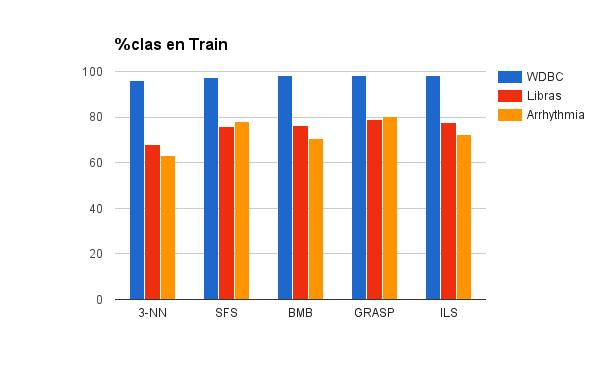
\includegraphics[width=0.7\textwidth]{train}
\caption{Tasa de acierto en el conjunto train} \label{fig:train}
\end{figure}

\begin{figure}[H]
\centering
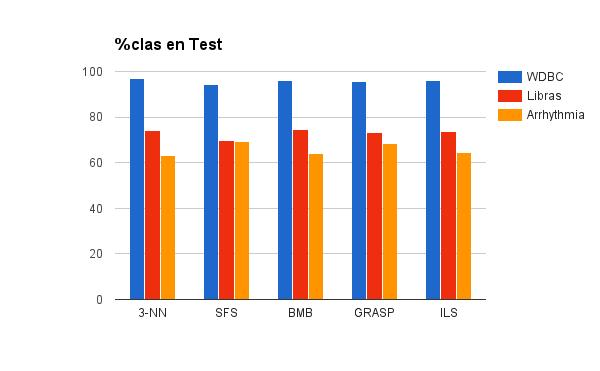
\includegraphics[width=0.7\textwidth]{test}
\caption{Tasa de acierto en el conjunto test} \label{fig:test}
\end{figure}

\begin{figure}[H]
\centering
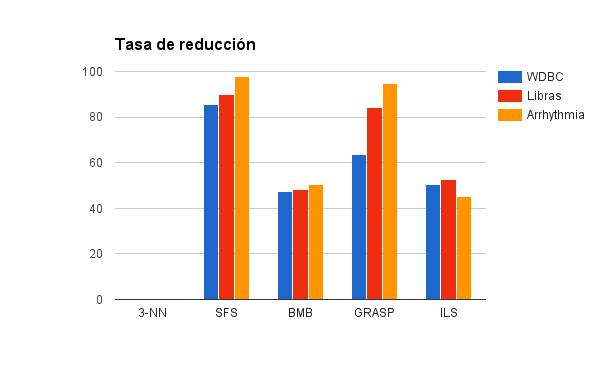
\includegraphics[width=0.7\textwidth]{reduccion}
\caption{Tasa de reducción} \label{fig:reduccion}
\end{figure}

\begin{figure}[H]
\centering
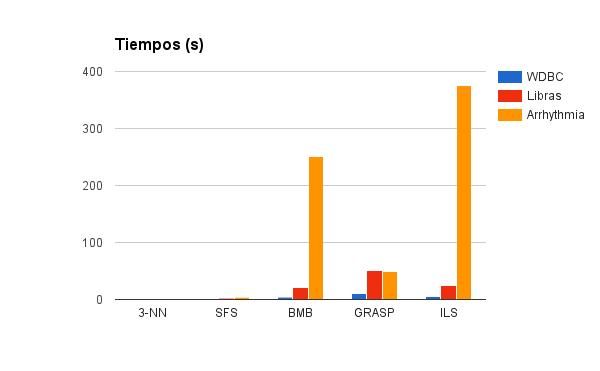
\includegraphics[width=0.7\textwidth]{tiempos}
\caption{Tiempo en segundos} \label{fig:tiempos}
\end{figure}

En este caso la condición de parada es para todos los algoritmos la misma (excepto para \texttt{SFS}), repetir el bucle interno 25 veces, por lo que el tiempo variará según lo que cada algoritmo haga en ese bucle interno.\\
En un principio podemos pensar que tiene sentido que el que menos tiempo tarde, entre \texttt{BMB}, \texttt{GRASP} e \texttt{ILS}, sea \texttt{BMB}, ya que lo único que repite 25 veces es la generación de una solución aleatoria inicial y la optimización de cada solución aleatoria con el método de \texttt{Búsqueda Local}, que de la práctica pasada, era el que menos tardaba. Después, \texttt{ILS} lo que hace es añadir a \texttt{BMB} una mutación de la mejor solución encontrada hasta el momento antes de optimizarla con \texttt{Búsqueda Local}, es decir, que cambia las últimas 24 generaciones aleatorias de \texttt{BMB} por mutaciones, por lo que los tiempos deberían ser un poco mayores pero parecidos (teniendo en cuenta que se tarda más en mutar que en generar aleatoriamente). Por último, el algoritmo \texttt{GRASP} es el más complicado en el sentido de que tiene más carga computacionalmente en principio, ya que lo que se repite 25 veces es una modificación del algoritmo \texttt{greedy} básico en el que en vez de coger la mejor característica en cada paso se elige una dentro de un cierto umbral de calidad y posteriormente se optimiza con \texttt{Búsqueda Local}, por lo que debería ser el que más tiempo tardara.\\
Esto es así efectivamente en las bases de datos con pocas características, como en Wdbc con 30 características o en Libras con 91 características, donde los tiempos son parecidos unos a otros. Sin embargo, para arritmia, donde tenemos 271 características, \texttt{GRASP} tarda bastante menos que \texttt{BMB} e \texttt{ILS}: \texttt{GRASP} tarda 49 segundos de media, \texttt{BMB} alrededor de 4 minutos de media e \texttt{ILS} más de 6 minutos de media por partición. De hecho, además, \texttt{GRASP} tarda un poco menos en arritmia que en Libras, como podemos ver en la gráfica de tiempos, lo que no pasa para ningún otro algoritmo.\\
Esto puede ser debido a que con la solución aleatoria con la que se empieza en \texttt{GRASP} ya no se encuentra mucha más mejora porque hay características que no influyen a la hora de elegir clase, de modo que la parte \texttt{greedy} modificada termina pronto dejando una solución bastante buena que la \texttt{Búsqueda Local} tampoco es capaz de mejorar mucho más (recordemos que la \texttt{Búsqueda Local} se queda en el primer óptimo local que encuentra, con lo que si ya estamos cerca de uno, no tardará en llegar a él), de forma que las \texttt{Búsquedas Locales} que hace \texttt{GRASP} duran menos que las que hacen \textit{BMB} e \texttt{ILS}, ya que en \texttt{BMB} hay que optimizar una solución aleatoria que no tiene por qué ser buena y en \textit{ILS} hay que optimizar una mutación, que ha podido quedar lejos de un óptimo local, y de hecho según los tiempos, vemos que en efecto queda lejos de un óptimo local.\\

Obviamente, todos tardan más que el algoritmo de comparación \texttt{SFS} ya que este sólo se repite una vez y no tiene optimización posterior (tampoco tendría sentido ya que hemos ido eligiendo características hasta que dejamos de obtener mejora).\\

Entrando ahora en comparar las tasas de acierto en el conjunto de train entre todos los algoritmos, \texttt{GRASP} es el que mejor tasa obtiene siempre, aunque con menos diferencia en Wdbc, hay más de un punto de diferencia en libras y casi dos en arritmia. Los demás algoritmos hay unos que funcionan mejor que otros según la base de datos, como \texttt{BMB}, que funciona mejor en Wdbc que \texttt{ILS}, aunque en realidad no hay mucha diferencia, mientras que \texttt{ILS} sí queda más de un punto por encima en Libras y casi dos en Arritmia, aunque en Arritmia tanto \texttt{ILS} como \texttt{BMB} quedan por debajo más de 5 puntos del \texttt{SFS}.\\

En cuanto a la tasa de acierto en test varía un poco con respecto a lo comentado para train, ya que ahora \texttt{GRASP} sólo tiene la mejor tasa en Arritmia, mientras que \texttt{BMB} es el que mejor tasa tiene para Wdbc y Libras, aunque las diferencias son menores que para los conjuntos de train. \texttt{SFS} es peor que \texttt{BMB}, \texttt{ILS} y \texttt{GRASP} excepto en Arritmia, donde sólo queda por debajo de \texttt{GRASP}, cuando en \texttt{SFS} estamos añadiendo características hasta que no hay mejora mientras que en \texttt{BMB} e \texttt{ILS} se comienza con soluciones aleatorias, lo que nos lleva a pensar que importa el orden en el que se elijan las características y en el \texttt{SFS} siempre se escoge primero la que más ganancia da, que es algo que no hace \texttt{GRASP} y de hecho este tiene tasas mejores.\\

En cuanto a la tasa de reducción, es normal que todas se queden por debajo del \texttt{SFS} por lo que acabamos de comentar y que el siguiente con mayor tasa de reducción sea \texttt{GRASP} que va añadiendo también característica a característica, mientras que el resto de algoritmos si tienen una característica que no esté aportando nada (o incluso está perjudicando) no nos estamos preocupando en eliminarla y tendrán más características al partir de soluciones aleatorias.\\

Con respecto al 3NN al principio parece raro que tenga menos tasa de acierto que los demás (en la mayoría de los casos) puesto que está considerando todas las características. Sin embargo como acabamos de comentar, no todas las características tienen que ser buenas definiendo una clase, además de que puede haber ruidos que hayan afectado más a unas que a otras. Es por esto que es normal que tenga un poco menos de acierto y que no haya mucha diferencia entre las tasas de acierto para entrenamiento y para test y además que la de entrenamiento no sea mejor que la de test, puesto que en este algoritmo en realidad las dos serían de test ya que no estamos utilizando ninguno de los dos conjuntos para aprender al estar utilizando todas las características.\\

Con todo esto, si tuviéramos que elegir uno de estos algoritmos para este problema, sería \texttt{GRASP}, ya que es el que mejor relación tasa/tiempo tiene, sobre todo si tenemos bastantes características, que es donde más se nota, mientras que si hay pocas la diferencia es menor, pero éste algoritmo sigue siendo ligeramente mejor.

\section{Bibliografía}
\begin{enumerate}
\item Scipy para leer ficheros arff \href{arff http://docs.scipy.org/doc/scipy/reference/generated/scipy.io.arff.loadarff.html}{aquí}.
\item Documentación de numpy \href{http://docs.scipy.org/doc/numpy/user/index.html}{aquí}.
\item Ficheros para el 3NN \href{https://github.com/agarciamontoro/metaheuristics/tree/master/src/knnGPU}{aquí} (aunque se encuentran también en los ficheros de mi práctica para poder utilizarlos).
\end{enumerate}

\end{document}